\section{Desugaring}
\label{sec:desugar}

\name is built upon a thin-layer of sugar on top of
\bname~\cite{alpuimdisjoint}. \bname is a polymorphic language with subtyping,
and it was developed as an alternative to languages such as System $F_{<:}$ to
serve as a core language for OO languages. The choice of \bname is due to its
support for disjoint intersection types and disjoint polymorphism (used to model
subtyping and conflict detection), and the so-called merge construct (which is
used to model dynamic trait inheritance). The theoretical aspects of \bname
(including the formalization of the static and dynamic semantics, and the proofs
of type safety and coherence) were already studied in previous work. So they are
not a contribution of this paper and are not necessary to understand the
desugaring process.

The novelty in this section is to explain how to build a high-level OO
abstractions on top of the core constructs of \bname. In particular we focus on
how the trait system presented in this paper is built. The key idea behind trait
translation is inspired by the functional mixin semantics using open recursion,
which is proposed by~\citet{cook1989denotational} in an untyped setting.
However, our translation is done in the context of a statically-typed
programming language, which is exactly why conflicts can be \textit{statically}
detected in traits.

\subsection{A Brief Introduction to \bname}
The syntax of our core language \bname is shown in Figure~\ref{fig:synax-fi}.

\paragraph{Types}
Apart from normal type constructs, the main novelty are two constructs used to
support disjoint intersection types and disjoint polymorphism: intersection
types $[[A & B]]$ and disjoint (universal) quantification $[[ forall ( a ** A )
. B ]]$. \bname also includes singleton record types $[[{ l : A}]]$ and type
applications $[[ T [ B1 , .. , Bn ] ]]$.

\paragraph{Terms}
In correspondence with types, terms include merges $[[E1 ,, E2]]$, abstraction
of type variables over terms $[[blam ( a ** A ) . E]]$, applications of terms to
types $[[E A]]$, and singleton records $[[ { l = E } ]]$. Record operations are
projections $[[E.l]]$ and exclusions $[[E -- { l : A }]]$.

\paragraph{Type and term declarations}

For the convenience of writing large programs, we also support type and term
declarations. A type declaration declares a type constructor's name $T$, its
type parameters and its definition $A$. A term declaration declares a function's
name $f$, its parameter signatures, its result type $B$, and its function body
$e$. Although previous work does not have declarations, we do not think adding
them will cause any problems to the meta-theory of \bname. A careful study of
these additions is of course a good avenue for future work.

\paragraph{Syntactic sugar} Multi-field record types are encoded as
intersections of singleton record types, and multi-field records as merges of
singleton records.

% \bruno{I think we can omit most of the primitive types and operations
%   from the formal syntax. You should present the syntactic sugar for
%   (multi-field) records and record types in the figure.}
% \bruno{Briefly explain the key novel contructs: merge, big lambda }
% \bruno{Explain that declarations/programs are new, but we don't think
%   this will cause any programs to the meta-theory.}

\begin{figure}[t]
\centering
\begin{small}
\begin{tabular}{lrcl}
  Types  & $[[A]], [[B]]$ & ::= & $[[top]] \mid [[Int]] \mid [[A -> B]] \mid [[A & B]] \mid  [[{ l : A }]] \mid [[a]] \mid [[forall ( a ** A ) . B]] \mid [[ T [ B1 , .. , Bn ] ]]$ \\
  Expressions & $[[E]]$ & ::= & $[[()]] \mid [[N]] \mid [[x]] \mid [[\ x . E]] \mid [[E1 E2]] \mid [[blam ( a ** A ) . E]] \mid [[E A]] \mid [[E1 ,, E2]] $ \\
         & & $\mid$ & $[[{ l = E }]] \mid [[E . l]] \mid [[E -- { l : A }]] $ \\
  Programs & $[[pgm]]$ & ::= & $[[decl1 .. decln E]]$ \\
  Declarations & $[[decl]]$ & ::= & $[[ def f ( x1 : A1 ) .. ( xn : An ) : B = E ]] \mid [[ type T [ a1 , .. , an ] = A ]]$ \\ \\
\end{tabular}
\begin{tabular}{llll}
  Record types & $[[ { l1 : A1 , ... , ln : An } ]] $ & := & $[[ { l1 : A1} & ... & { ln : An } ]]$ \\
  Records &  $[[ { l1 = E1 , ... , ln = En } ]] $ & := & $ [[ { l1 = E1 } ,, ... ,, { ln = En } ]]$
\end{tabular}
\end{small}
\caption{\bname syntax and syntactic abbreviations}
\label{fig:synax-fi}
\end{figure}

\subsection{Desugaring Traits}

\paragraph{Trait declarations}

The left part of Figure~\ref{fig:trans-trait} presents the translation of trait
declarations. Essentially traits are translated into term declarations, with
methods becoming record fields. The self-reference is adjusted to be the last
parameter of the declaration. For example
\begin{lstlisting}
trait point(x : Int, y: Int) { self : Point =>
  def x = x
  def y = self.x }
\end{lstlisting}
becomes
\begin{lstlisting}
def point (x : Int) (y : Int) (self : Point) = { x = x , y = self.x }
\end{lstlisting}
Now it is clear that \lstinline{self} is not a special keyword: it can have any
name.

% To account for the call-by-value semantics of the
% target language, the type of the self-reference $s$ has become a thunk
% \lstinline[mathescape=true]{T -> $A_0$}, and the occurrences of the
% self-reference \lstinline{s} in the trait body are replaced by \lstinline{s()}.


\paragraph{Instantiation of traits}

The right part of Figure~\ref{fig:trans-trait} shows the translation of trait
instantiation. Specifically, the self-reference gets passed to each trait $m_1$
to $m_n$, as each of them is an open term after translation. The results are
then merged to form a new term. \lstinline{new} instantiates a trait by
taking the \textit{lazy fixpoints} of the resulting term. For example,
\lstinline{new[Point] point(3,4)} is translated into \lstinline{let self : Point = point 3 4 self in self}.
\name has a lazy (and possibly recursive) \lstinline{let} construct.


% Lazy fixpoints are implemented in \name using the built-in \lstinline{let}
% construct (possibly recursive), which employs call-by-name semantics. It is
% possible to choose call-by-value, then the type of the self-reference would
% become a thunk (e.g., \lstinline$T -> Point$) to prevent premature evaluation.


\paragraph{The type for traits}

\lstinline[mathescape=true]{Trait[$T_1, T_2$]} denotes the type of those traits
which provide an interface described by the type $T_2$ with dependency on $T_1$.
In fact, it is simply translated into $T_1 \rightarrow T_2$.

\begin{figure}[t]
  \centering
  \begin{tabular}{l|l}

\begin{lstlisting}[mathescape=true]
trait m ($x_1 : A_1$, ..., $x_n : A_n$)
  inherits $a_1$ & ... & $a_m$ { $s : A_0$ =>
  def $m_1$(..) = $e_1$
  ..
  def $m_s$(..) = $e_s$ }
\end{lstlisting} &

\begin{lstlisting}[mathescape=true]
new[A] $m_1$ & ... & $m_n$
\end{lstlisting}  \\

    $\rightsquigarrow$  & $\rightsquigarrow$ \\

\begin{lstlisting}[mathescape=true]
def m $(x_1 : A_1)$ ... $(x_n : A_n)$ $(s : A_0)$
  = $a_1$(s) ,, ... ,, $a_m$(s) ,,
{ $m_1$ = \(..) -> $e_1$
, ..
, $m_s$ = \(..) -> $e_s$ }
\end{lstlisting} &


\begin{lstlisting}[mathescape=true]
let self : A =
  $m_1$(self) ,, ... ,, $m_n$(self)
in self
\end{lstlisting}
  \end{tabular}
  \caption{Translations of trait declaration (left) and trait instantiation (right)}
\label{fig:trans-trait}

\end{figure}



\section{Implementation and Discussion}

The \name prototype implementation is structured around a typed core language
(\bname with some extensions). The overall implementation is unremarkable, as it
closely follows the semantics presented by~\citet{alpuimdisjoint}. It consists
of 3 phases: 1) The desugaring phase (cf. Section~\ref{sec:desugar}) takes an
abstract syntax tree (AST) generated by the parser, and returns a \bname
expression. Trait-related constructs disappear after this phase; 2) the type
checking phase then takes a \bname expression from the previous phase, it infers
and checks its type, and in the meantime, produces an expression in the target
language; and 3) the target expression (call-by-name pure untyped lambda
calculus) then enters the final phase, and is executed by a simple interpreter.

% The main component of the implementation is an
% elaborating type-checker, which takes a \bname expression, checks it, and
% produces another expression in the target language. The final expression is then
% directly executed by an interpreter. We chose call-by-value untyped lambda
% calculus as the target language. Since we focus on the implementation, and types
% are irrelevant after type checking, the untyped lambda calculus is a suitable choice
% with minimal syntax.


The type checker is the most involved component in the pipeline. It contains a
(coercive) subtyping procedure and a disjointness checker, both of which are the
most critical parts in \name. In regard to the subtyping rules, in addition to what have
been presented~\citep{alpuimdisjoint}, we have an additional rule, which we
found helpful for enabling the composition of Object Algebras. For brevity, we
only show a simplified version below: \ottusedrule{\ottdruleSubXXR{}} By this
rule, one can derive for example,
$$
[[ { l : Int -> String} & { l : Bool -> Bool}]] <: [[ { l : Int & Bool -> String & Bool}]]
$$
We believe this rule would not endanger the type
system, as it is orthogonal to the other subtyping rules. Besides, our
preliminary meta-theory study shows that the new subtype system enjoys the same
properties as before.

The prototype implementation is written in just 1400 lines of Haskell code.

% \begin{figure}[t]
%   \centering
%   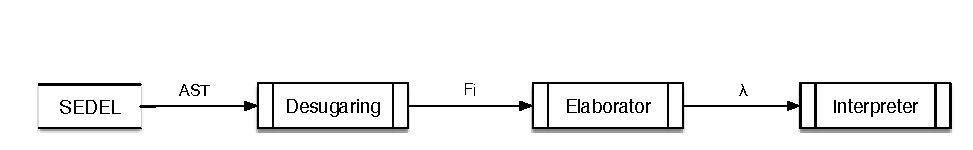
\includegraphics[scale=0.9]{pipeline.eps}
%   \caption{The pipeline of \name}
%   \label{fig:pipeline}
% \end{figure}